\chapter{Result}
Now we can use our method to determine $dS/dt$, $Pre$, $ET$ and $R$. After that, we can combine these results and discuss the trend of water storage in Ob basin and the reason for it.
\section{Total water storage anomaly}
As mentioned in chapter 3, 4 time series (CSR, GFZ, ITSG, JPL) of TWSA from Apr. 2002 to May. 2020 are handled in this work. By using the method in \autoref{sec:Gaussmarkov}, these four time series can be summarized into one time series \autoref{fig:twsa}. It is shown that the TWSA increases in summer and decreases in winter annually. As can be assumed in this figure, the TWSA remains unchanged before 2010, between 2010 and 2012 the TWSA decreased and then it increased till at least 2017.   \\
\begin{figure}[htbp]\centering
	\begin{minipage}[t]{0.85\textwidth}
		\centering
		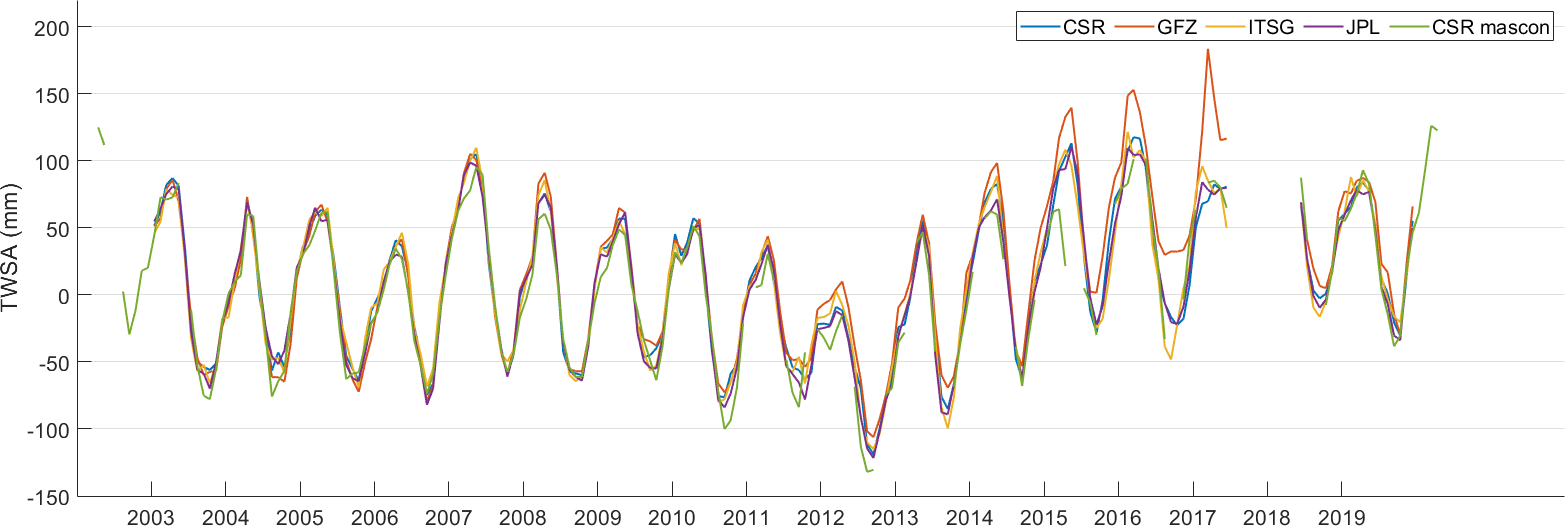
\includegraphics[width=1\textwidth]{TWSAall} % Datei in "bilder/" bei LaTeX: eps, bei PDFLaTeX: jpg (o.ä.) 
	\end{minipage}
	\begin{minipage}[t]{0.85\textwidth}
		\centering
		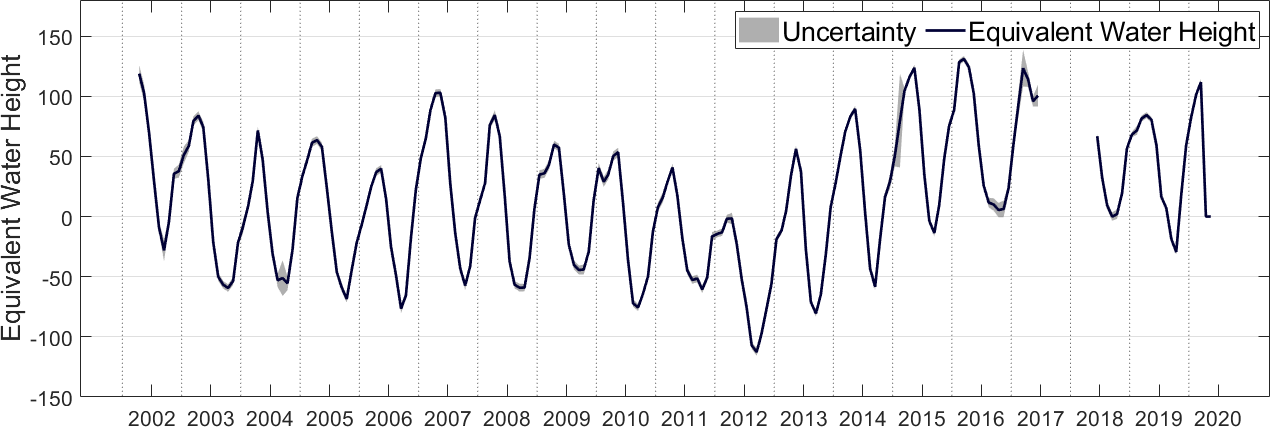
\includegraphics[width=1\textwidth]{EWH} % Datei in "bilder/" bei LaTeX: eps, bei PDFLaTeX: jpg (o.ä.) 
	\end{minipage}
	\caption{TWSA generated from different data centers (top) generate one summarized TWSA time series (bottom) from Jan.2003 to Dec.2019}
	\label{fig:twsa}
\end{figure}\\
By using the methods in \autoref{eq:dsdt} and \autoref{sec:changpoint} 2 abrupt change in the deviation of TWSA are found. The time of these two points are October of 2012 and November of 2015, which proves the assumption of positive trend above, while the negative trend between 2010 and 2012 can not determined. With this 2 points the whole time series can thus divide into 3 periods \autoref{tab:3periods}. Note that Jan. 2013 and Jan. 2016 are chosen to be the split points because we need the annual behavior of the TWSA. 
\begin{figure}[htbp]\centering
	\begin{minipage}[t]{0.7\textwidth}
		\centering
		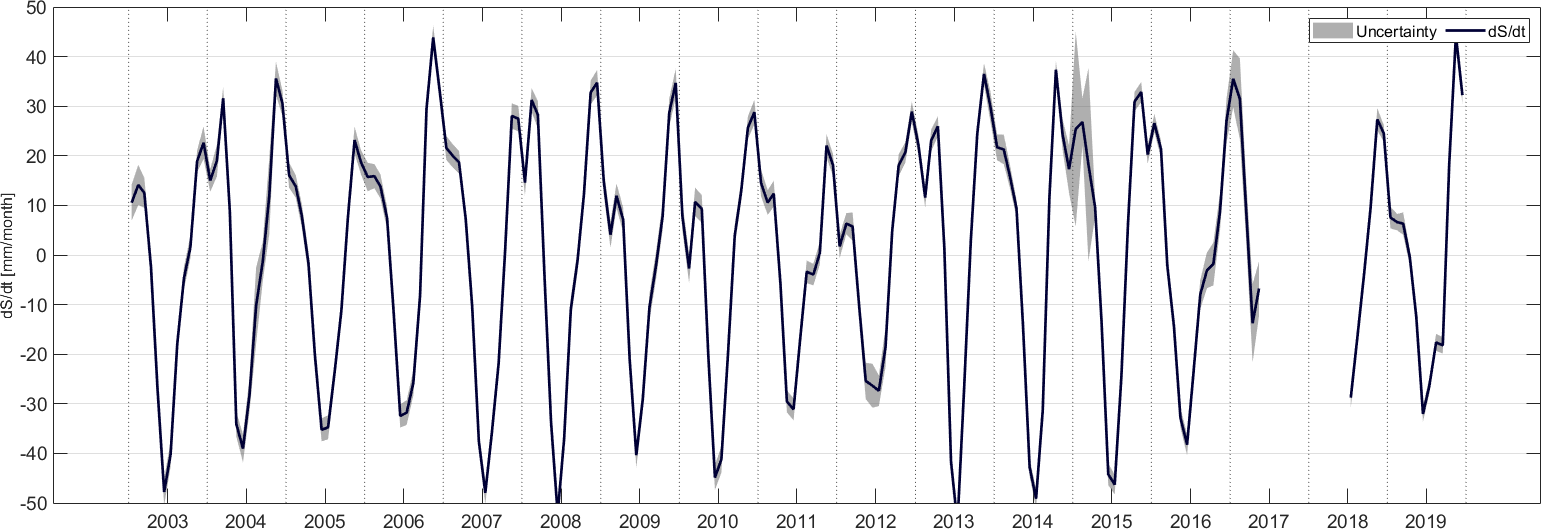
\includegraphics[width=1\textwidth]{dSdt} % Datei in "bilder/" bei LaTeX: eps, bei PDFLaTeX: jpg (o.ä.) 
	\end{minipage}
	\begin{minipage}[t]{0.7\textwidth}
		\centering
		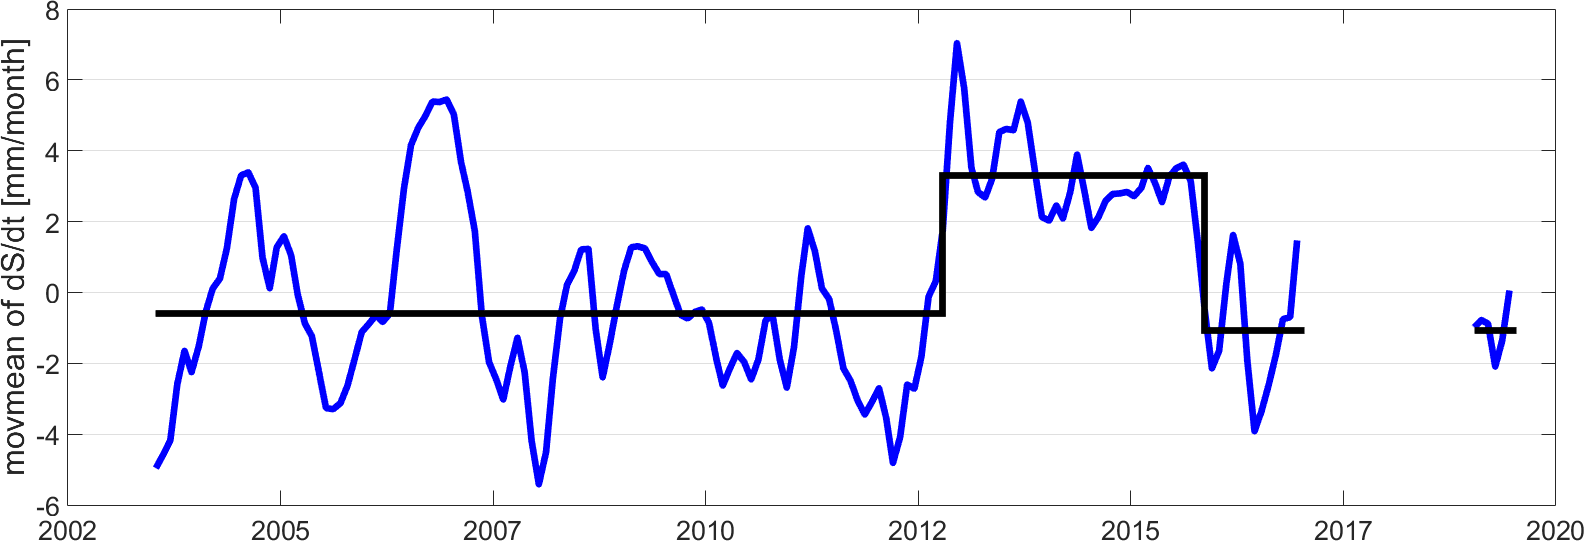
\includegraphics[width=1\textwidth]{dSdtmovmean} % Datei in "bilder/" bei LaTeX: eps, bei PDFLaTeX: jpg (o.ä.) 
	\end{minipage}
	\caption{the derivation of TWSA (top) and the abrupt change in the moving average (bottom)}
	\label{fig:dsdt}
\end{figure}
\begin{table}[htbp] \centering
	\begin{tabular}{|l|}
		\hline
		Jan. 2003 - Dec. 2012   \\ \hline 
		Jan. 2013 - Dec. 2015	\\ \hline 
		Jan. 2016 - Dec. 2019	\\ \hline 
	\end{tabular}
	\caption{3 periods divided by split points}
	\label{tab:3periods}
\end{table}\\
After that, the mean $dS/dt$ along with the RMSE in these 3 periods can be calculated \autoref{fig:dsdtnum}, it is shown that in the first and the third period $dS/dt$ are nearly 0, while in the second period the number is much higher, which means from Jan. 2013 to Dec. 2015 the total water storage gained in Ob basin area.
\begin{figure}[htbp]
	\centering
	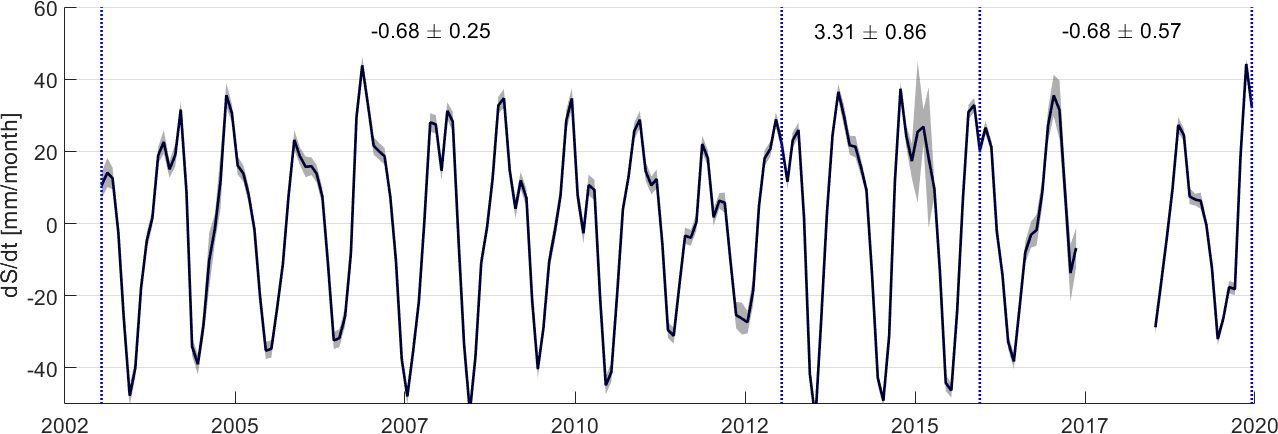
\includegraphics[width=0.7\textwidth]{dSdtwithnum} 
	\caption{mean value of dS/dt and RMSE in 3 periods} 
	\label{fig:dsdtnum}
\end{figure}\\
As mentioned in chapter 2, the Ob river basin contains a big area. Therefor, it's necessary to confirm, that the behavior of total water storage change is similar among the basin. 
\begin{figure}[htbp]\centering
	\begin{minipage}[t]{0.3\textwidth}
		\centering
		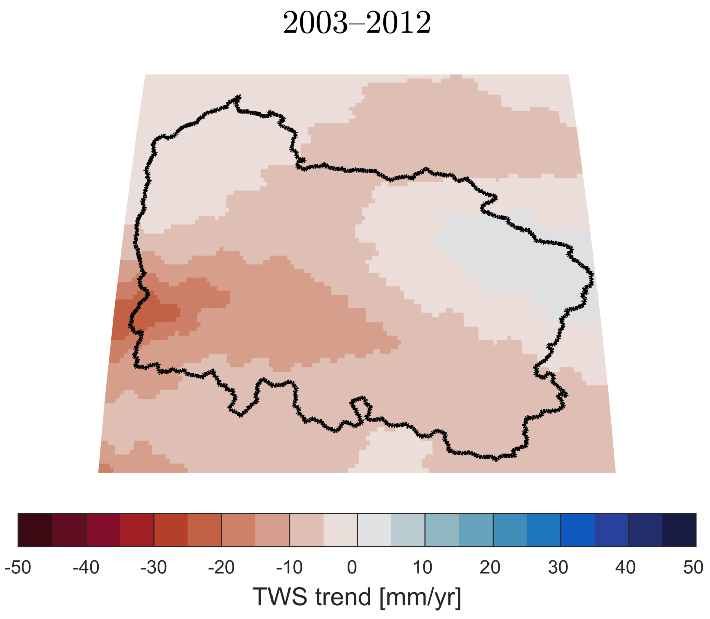
\includegraphics[width=1\textwidth]{trend1} % Datei in "bilder/" bei LaTeX: eps, bei PDFLaTeX: jpg (o.ä.) 
	\end{minipage}
	\begin{minipage}[t]{0.3\textwidth}
		\centering
		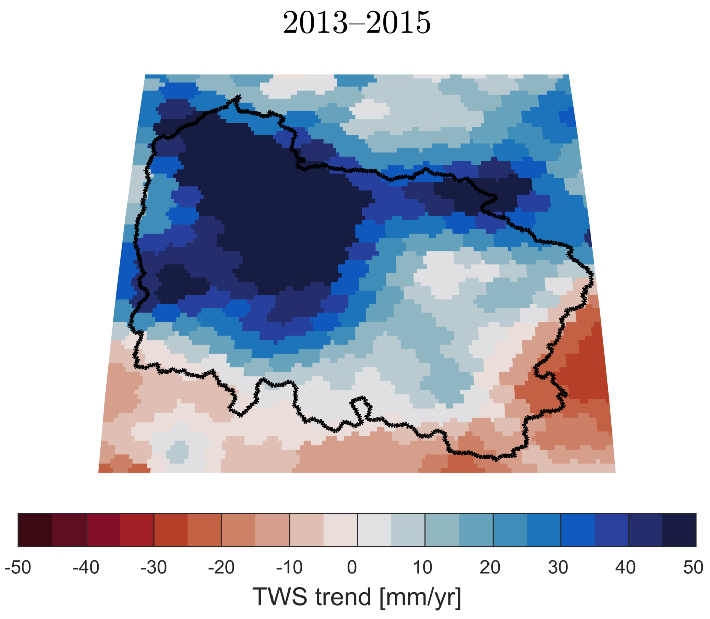
\includegraphics[width=1\textwidth]{trend2} % Datei in "bilder/" bei LaTeX: eps, bei PDFLaTeX: jpg (o.ä.) 
	\end{minipage}
	\begin{minipage}[t]{0.3\textwidth}
		\centering
		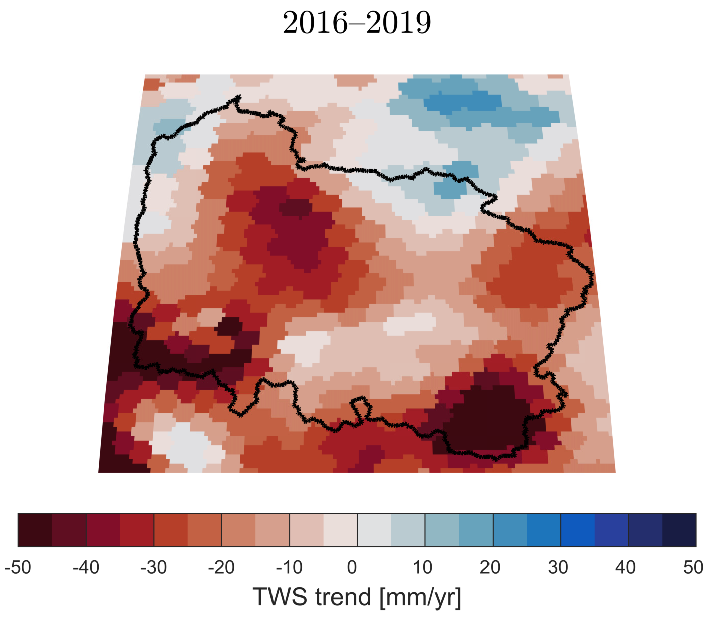
\includegraphics[width=1\textwidth]{trend3} % Datei in "bilder/" bei LaTeX: eps, bei PDFLaTeX: jpg (o.ä.) 
	\end{minipage}
	\caption{spatial TWS change of Ob river basin in each period}
	\label{fig:twsspatial}
\end{figure}\\
\clearpage
\section{Precipitation}
It was mentioned in chapter 3 that precipitation data from 9 datasets are processed and one time series with uncertainty can be generated by summarizing them \autoref{fig:prenum} just as before. The uncertainty are calculated using methods mentioned in \autoref{sec:error}.
\begin{figure}[htbp]\centering
	\begin{minipage}[t]{0.9\textwidth}
		\centering
		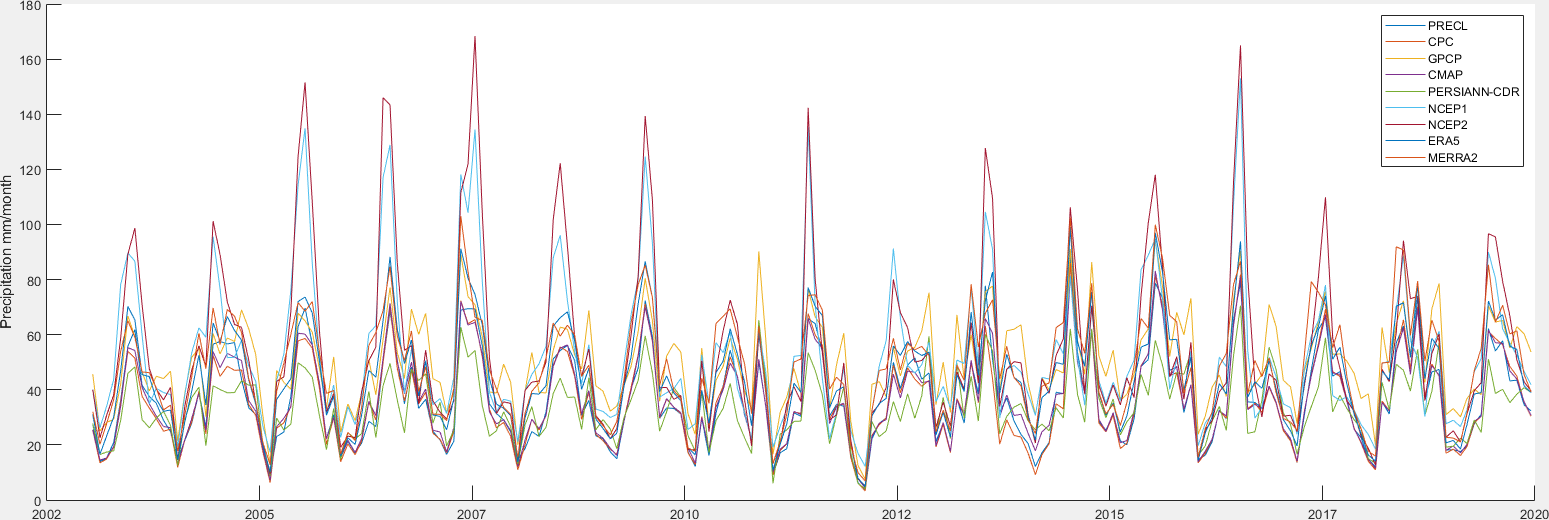
\includegraphics[width=0.9\textwidth]{precenter} % Datei in "bilder/" bei LaTeX: eps, bei PDFLaTeX: jpg (o.ä.) 
	\end{minipage}
	\begin{minipage}[t]{0.9\textwidth}
		\centering
		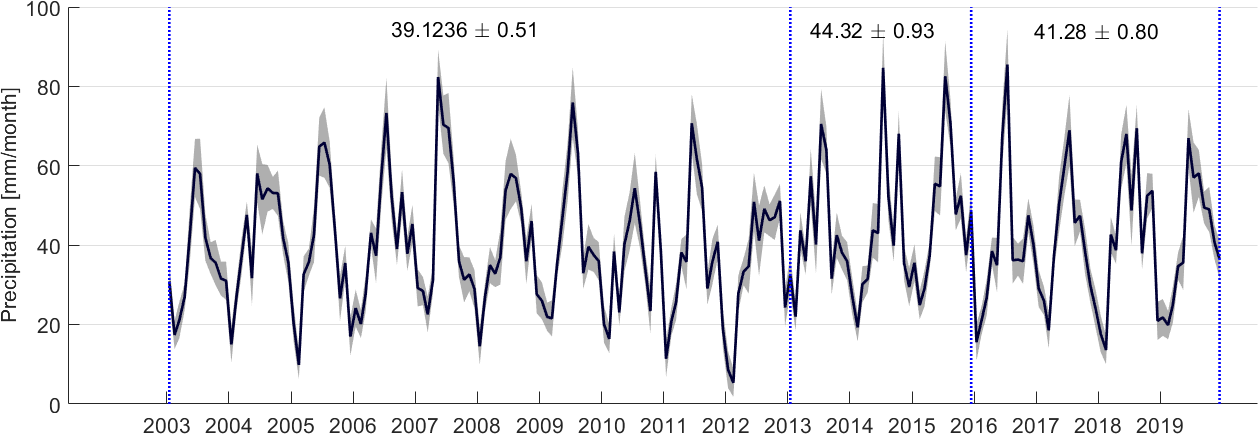
\includegraphics[width=0.9\textwidth]{precipitationwithnumber} % Datei in "bilder/" bei LaTeX: eps, bei PDFLaTeX: jpg (o.ä.) 
	\end{minipage}
	\caption{all precipitation datasets (top) are summarized into one time series, the mean precipitation with RMSE in 3 periods are calculated (bottom)}
	\label{fig:prenum}
\end{figure}\\
As what was done for $dS/dt$, the precipitation are also divided into 3 periods, the mean value and RMSE shows that in the second periods the amount of precipitation in this area is $5.2\ut{mm/month}$ bigger than the first period. The precipitation in the third period, however, is less than the second period but still more than the first period.\\\\
The spatial analyze of precipitation is also presented \autoref{fig:spatialpre}, 
\begin{figure}[htbp]\centering
 	\centering
 	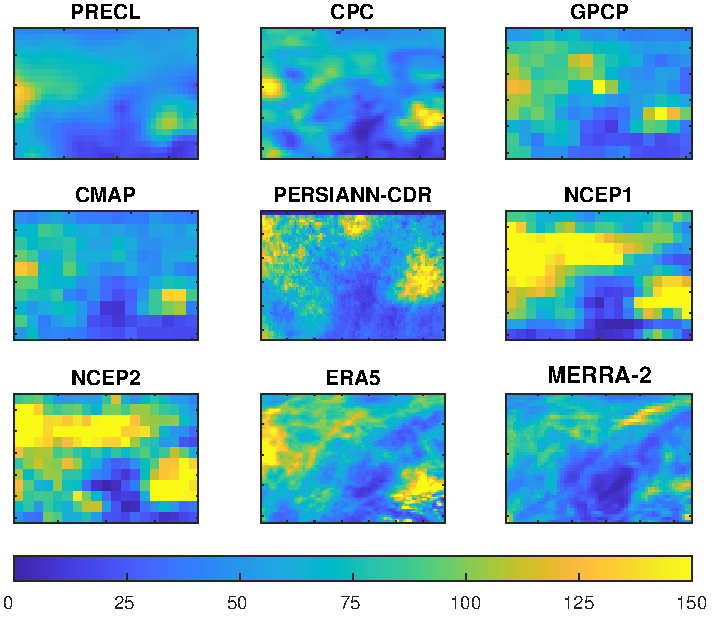
\includegraphics[width=0.9\textwidth]{Pre_spatial_June2003} % Datei in "bilder/" bei LaTeX: eps, bei PDFLaTeX: jpg (o.ä.) 
 	\caption{spatial change of precipitation in Ob river basin using different datasets in June of 2003} 
 	\label{fig:spatialpre}
\end{figure}
\clearpage
% all precipitation in one 
\section{Evapotranspiration}
Just as precipitation, the evapotranspiration is presented temparally and the time series is split into 3 periods. The mean value along with RMSE are also calculated. From \autoref{fig:etnum} we can see that the evapotranspiration reaches the summit in summer but nearly disappear in the winter. The results of evapotranspiration is similar to what we see in precipitation: it increases in the second period by $1.54 \ut{mm/month}$ and decreases after Dec. 2015 and it didn't go back to the original level in the first period like precipitation. It should also be noted that evapotranspiration has not increased that much in the second period as in precipitation, which follows the rules of water cycle.
\begin{figure}[htbp]\centering
	\begin{minipage}[t]{0.9\textwidth}
		\centering
		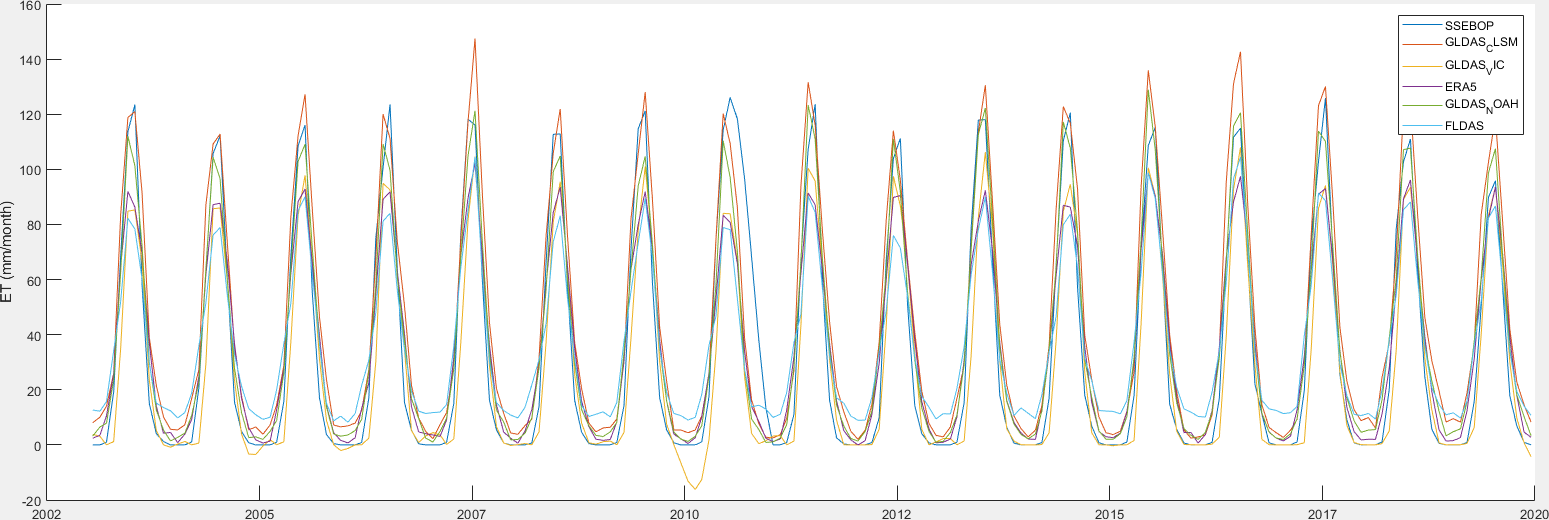
\includegraphics[width=0.9\textwidth]{etcenter} % Datei in "bilder/" bei LaTeX: eps, bei PDFLaTeX: jpg (o.ä.) 
	\end{minipage}
	\begin{minipage}[t]{0.9\textwidth}
		\centering
		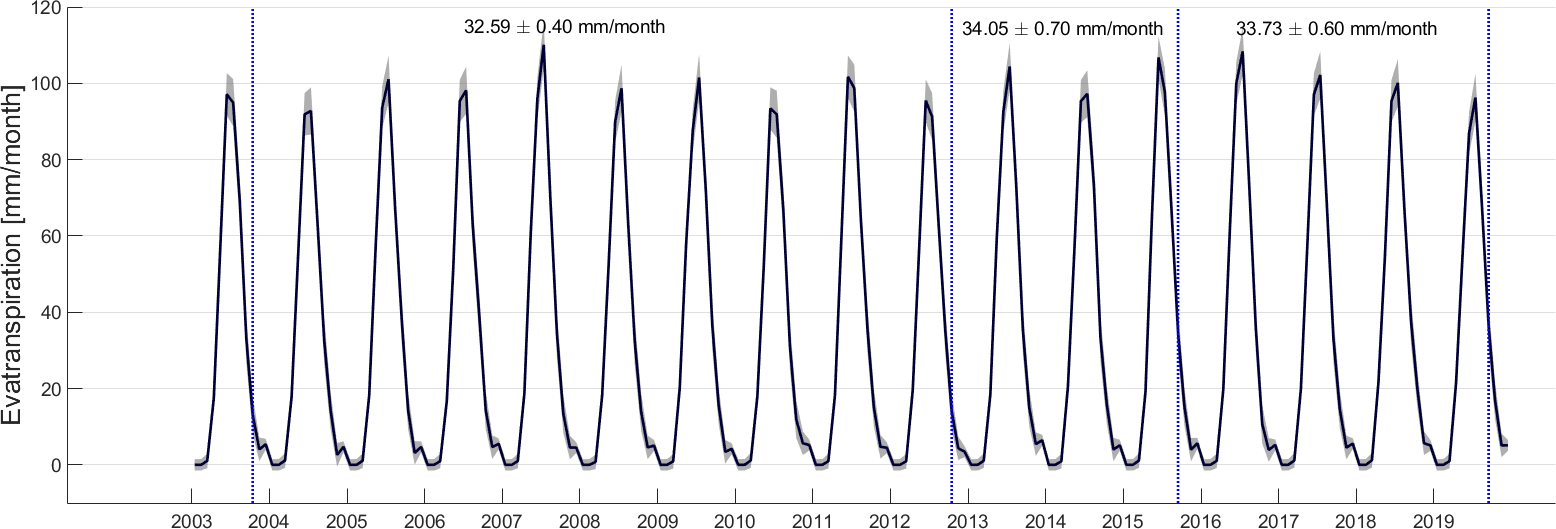
\includegraphics[width=0.9\textwidth]{etall} % Datei in "bilder/" bei LaTeX: eps, bei PDFLaTeX: jpg (o.ä.) 
	\end{minipage}
	\caption{all evapotranspiration datasets (top) are summarized into one time series, the mean precipitation with RMSE in 3 periods are calculated (bottom)}
	\label{fig:etnum}
\end{figure}\\
The spatial analyze of evapotranspiration is also made, like precipitation \autoref{fig:spatialet}
\begin{figure}[htbp]\centering
	\centering
	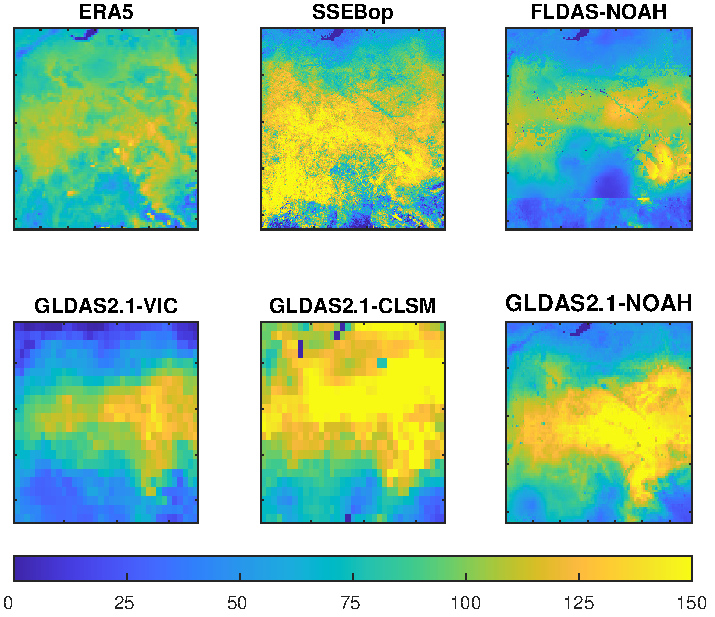
\includegraphics[width=0.9\textwidth]{ET_spatial_June2003} % Datei in "bilder/" bei LaTeX: eps, bei PDFLaTeX: jpg (o.ä.) 
	\caption{spatial change of evapotranspiration in Ob river basin using different datasets in June of 2003} 
	\label{fig:spatialet}
\end{figure}
\clearpage
\section{Runoff}
\subsection{Runoff from global datasets}
Like precipitation and evapotranspiration, Runoff data estimated from several models are provided and meanwhile the in-situ data till end of 2010 is available \autoref{fig:rcenter}. It can been seen that the differences between models and in-situ data are not small.  By calculating RMSE for these models the quality of them can be estimated. \autoref{tab:runofferror} provides the RMSE for all these datasets, the smallest RMSE is already bigger than 8\ut{mm/month}, which is hardly to trust for further analyze. 
\begin{figure}[htbp]\centering
	\centering
	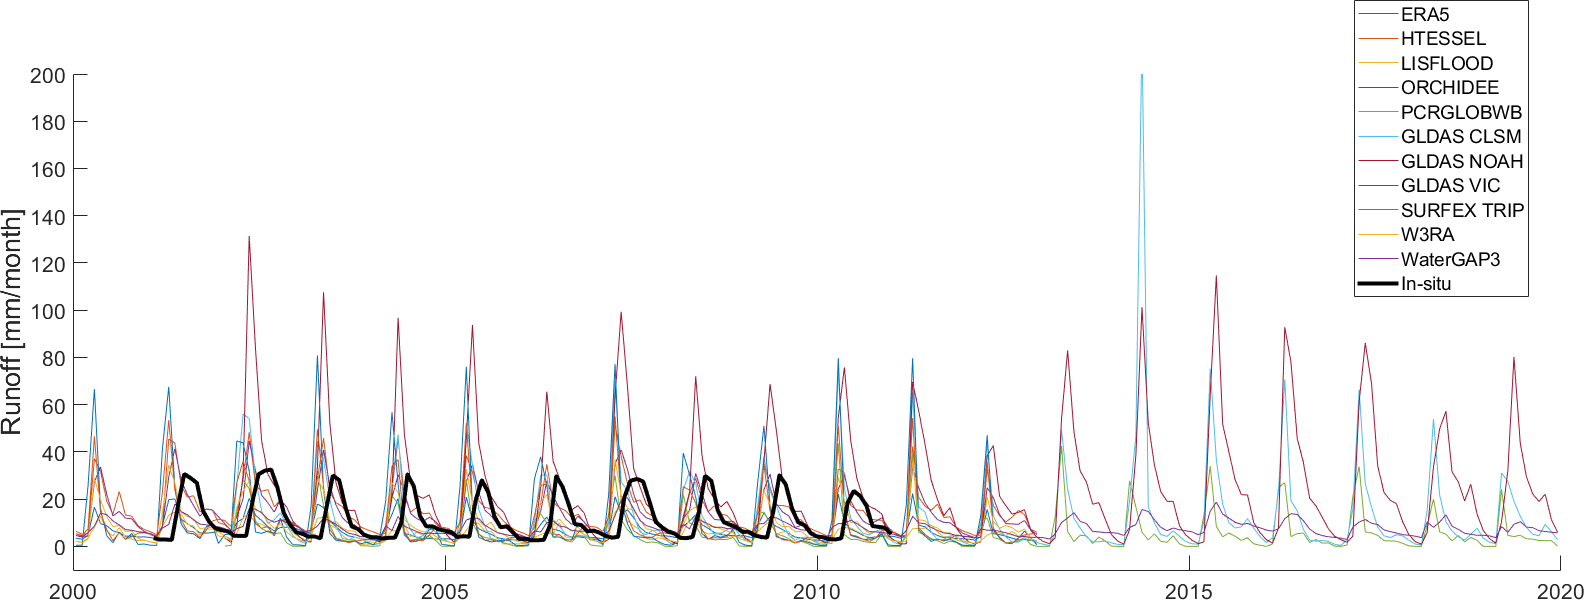
\includegraphics[width=0.9\textwidth]{runoffcenter} % Datei in "bilder/" bei LaTeX: eps, bei PDFLaTeX: jpg (o.ä.) 
	\caption{Runoff datasets, the black bold time series is the in-situ runoff} 
	\label{fig:rcenter}
\end{figure}
\begin{table}[htbp]\label{tab:rmse} \centering
	\begin{tabular}{|l|l|}
		\hline
		Datacenter  & RMSE (mm/month) \\ \hline
		ERA5        & 8.18  \\ \hline
		HTESSEL     & 10.40 \\ \hline
		LISFLOOD    & 11.92 \\ \hline
		ORCHIDEE    & 10.24 \\ \hline
		PCRGLOBWB   & 9.48  \\ \hline
		GLDAS CLSM  & 13.68 \\ \hline
		GLDAS NOAH  & 17.01 \\ \hline
		GLDAS VIC   & 25.95 \\ \hline
		SURFEX-TRIP & 22.05 \\ \hline
		W3RA        & 16.47 \\ \hline
		WaterGAP3   & 11.03 \\ \hline
	\end{tabular}
	\caption{RMSE for runoff datacenters}
	\label{tab:runofferror}
\end{table}\\
Then, if we take the CDF of the difference from those models and in-situ data and set 10\% of mean in-situ runoff as quantile \autoref{fig:rcdf} , it is shown that none of these datasets has achieved probability of 90\%. Therefor, the runoff would be estimated using satellite altimetry. 
\begin{figure}[htbp]
	\centering
	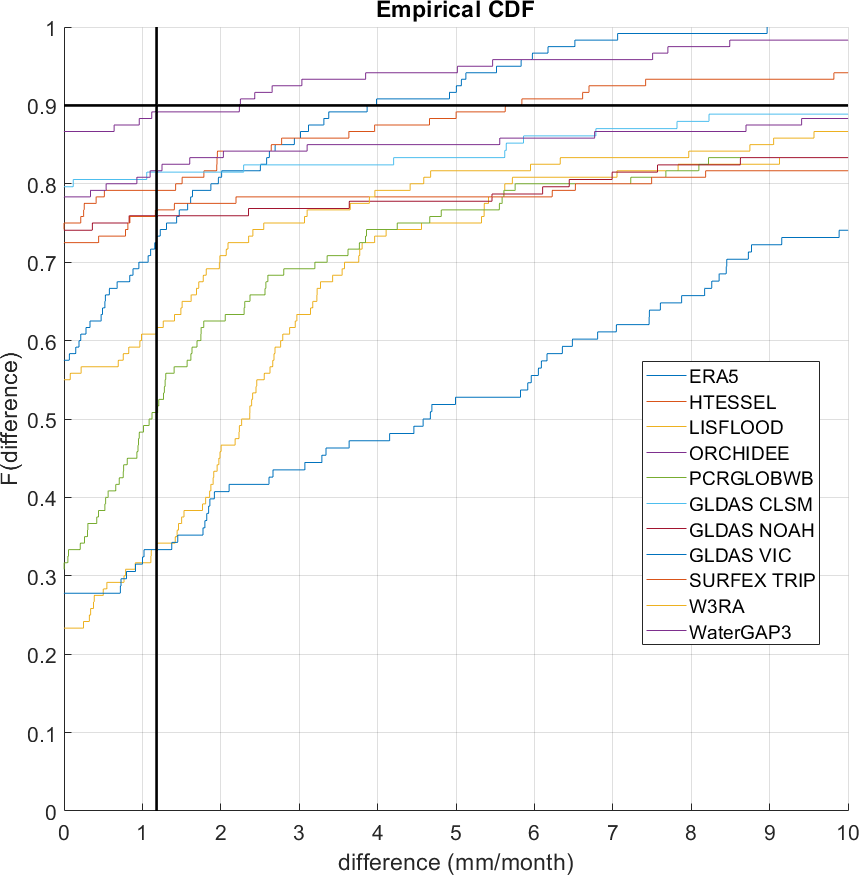
\includegraphics[width=0.6\textwidth]{rcdf} % Datei in "bilder/" bei LaTeX: eps, bei PDFLaTeX: jpg (o.ä.) 
	\caption{CDF of differences} 
	\label{fig:rcdf}
\end{figure}\\
\subsection{Estimating runoff using quantile function and satellite altimetry}
 The methods for runoff estimating is introduced in \autoref{sec:runoff}, \autoref{fig:waterlevel} presents water level time series from Envisat, SARAL and Sentinel. For each mission 2 virtual stations are chosen. In order to get an accurate runoff, water lever whose virtual station closer to Salekhard station are used to generated the final runoff. After combining all 3 time series from different space mission, an runoff time series from Jan. 2001 to Dec. 2019 is obtained \autoref{fig:runoff} (top, blue line). Noted that except the gap between Envisat and SARAL, other monthly gaps exists too, these gaps are filled with interpolation \autoref{fig:runoff} (top, red line). \\\\
 Then, as the precipitatin and evapotranspiration, the runoff time series is also divided into 3 periods \autoref{fig:runoff} (bottom) and RMSE is calculated from the method \autoref{sec:waterlevel}. It shows that the runoff in the first periods and in the second periods changes not much, but in the third periods the runoff has increased by about 2 mm/month. 
 \begin{figure}[htbp]
 	\centering
 	\begin{minipage}[t]{0.7\textwidth}
 		\centering
 		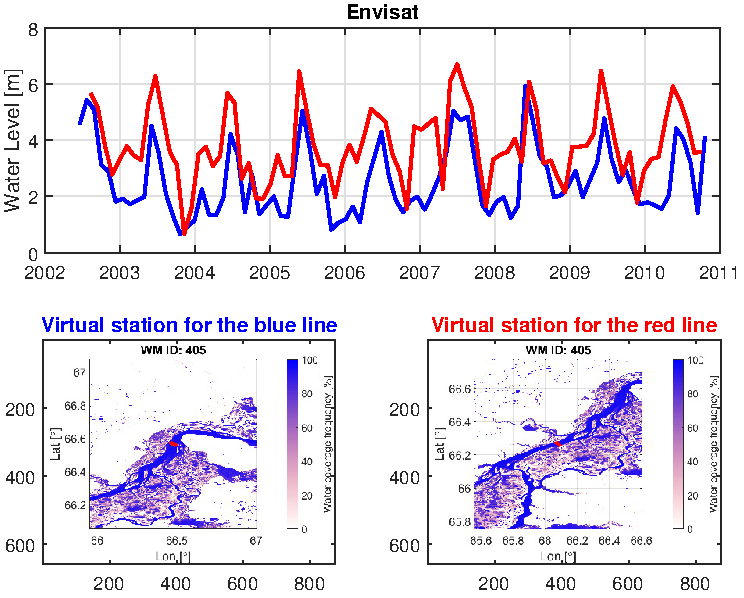
\includegraphics[width=0.8\textwidth]{Envisat_Ob} % Datei in "bilder/" bei LaTeX: eps, bei PDFLaTeX: jpg (o.ä.) 
 	\end{minipage}
 	\begin{minipage}[t]{0.7\textwidth}
 		\centering
 		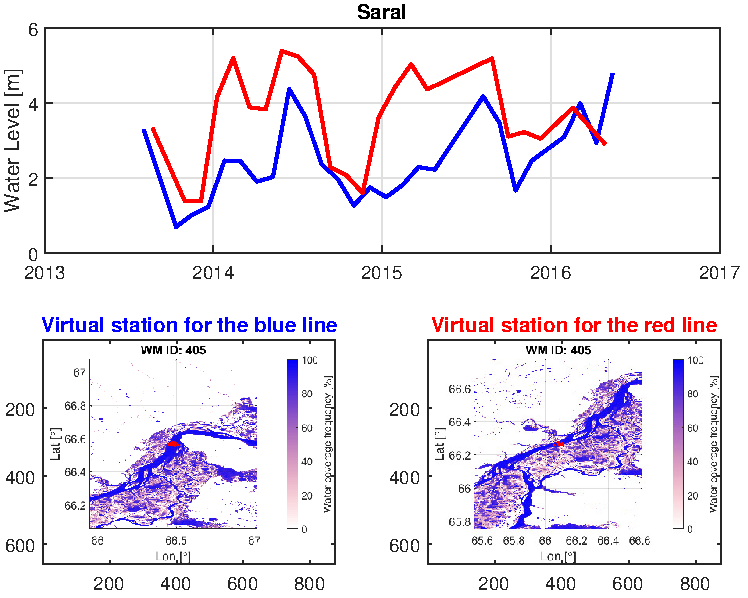
\includegraphics[width=0.8\textwidth]{Saral_Ob} % Datei in "bilder/" bei LaTeX: eps, bei PDFLaTeX: jpg (o.ä.) 
 	\end{minipage}
 \begin{minipage}[t]{0.7\textwidth}
 	\centering
 	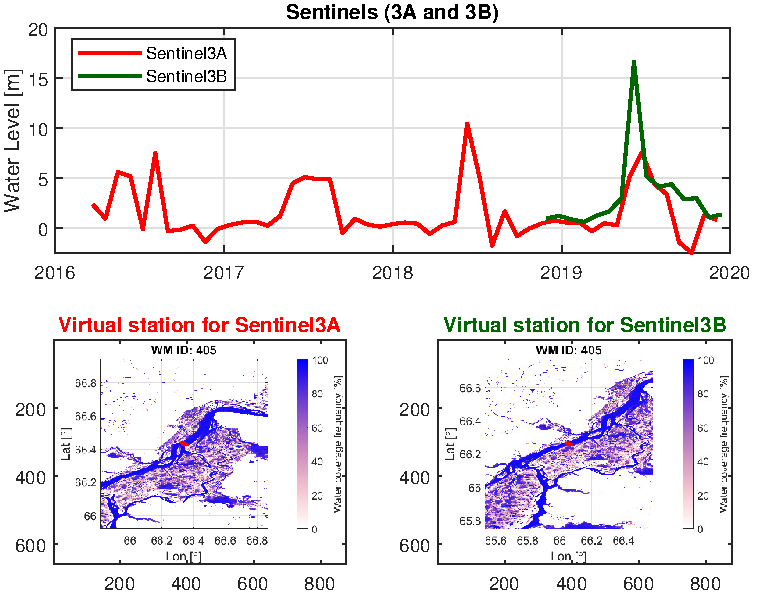
\includegraphics[width=0.8\textwidth]{Sentinels_Ob} % Datei in "bilder/" bei LaTeX: eps, bei PDFLaTeX: jpg (o.ä.) 
 \end{minipage}
 \caption{water level time series and the location of virtual station for different space mission}
 \label{fig:waterlevel}
 \end{figure}
\begin{figure}[htbp]
	\centering
	\begin{minipage}[t]{0.9\textwidth}
		\centering
		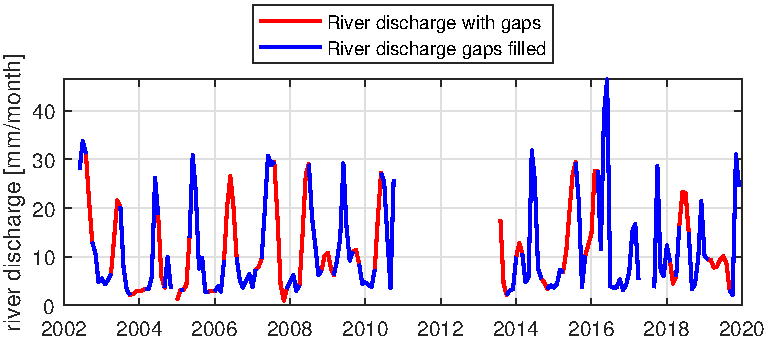
\includegraphics[width=1\textwidth]{Dis_Ob} % Datei in "bilder/" bei LaTeX: eps, bei PDFLaTeX: jpg (o.ä.) 
	\end{minipage}
	\begin{minipage}[t]{0.9\textwidth}
		\centering
		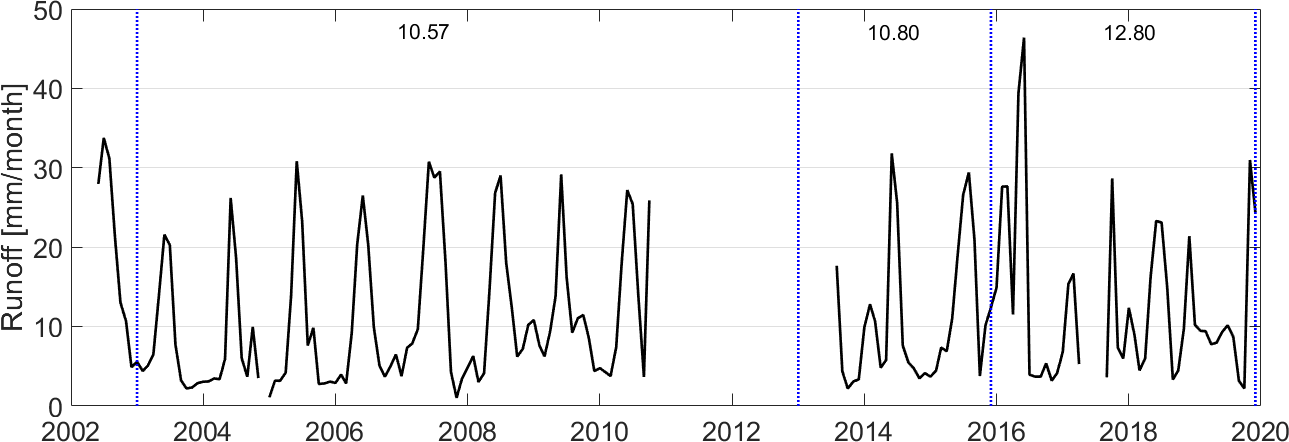
\includegraphics[width=1\textwidth]{runnumber} % Datei in "bilder/" bei LaTeX: eps, bei PDFLaTeX: jpg (o.ä.) 
	\end{minipage}
	\caption{runoff timeseries calculated from water level (top) and the mean value in 3 periods(bottom) }
	\label{fig:runoff}
\end{figure}
\clearpage
\section{Discussion about the quality}
Since the total water storage in the first period can be seen as stable, we take this period as the baseline for further analyze. Relative dS/dt, precipitaion, evapotranspiration and runoff numbers of other 2 period are obtained based on that. \\\\
In any case, the equation of terrestrial water balance \autoref{equa:waterbalence} has to be a true statement, which means the result of $Pre-dS/dt-ET-R$ should be 0. By setting results of both periods into this statement, it is shown that the results for the second period are proved while the results for the third periods are not ideal. This can be caused by the gap between GRACE and GRACE-FO. This gap is between Jul. 2017 and May. 2018, therefore, we only have full year data of 2016 and 2019 in this period. Though we tried linear regression to make the best use of what we have, this gap can still increase the instability of the final results because the period is not long enough. 
\begin{table}[htbp]\centering
	\begin{tabular}{|l|l|l|l|}
		\hline
		Period &  2003 - 2012 & 2013 - 2015 & 2016 - 2019  \\ \hline
		dS/dt            & $-0.68 \pm 0.25$     & $3.31 \pm 0.86$        & $-0.80 \pm 0.57$        \\ \hline
		Precipitaion               & $39.12 \pm 0.51$      & $44.32 \pm 0.93$       &$41.28 \pm 0.80$        \\ \hline
		evapotranspiration           & $32.59 \pm 0.38$       & $34.13 \pm 0.70$       & $33.78 \pm 0.6$        \\ \hline
		Runoff                     & $10.57  \pm 4.16$      & $10.80 \pm 4.16 $     & $12.80 \pm 4.16 $      \\ \hline
		\multicolumn{4}{|l|}{Based on the first period}                                         \\ \hline
		dS/dt           &             & $4.00 \pm 0.45$        & $-0.11 \pm 0.52$        \\ \hline
		Precipitaion               &             & $5.20 \pm 0.53$        & $2.15 \pm 0.61$         \\ \hline
		evapotranspiration           &             & $1.53 \pm 0.40$        & $1.19 \pm 0.46 $        \\ \hline
		Runoff                     &             & $0.23 \pm 2.94 $       & $2.23 \pm 2.94   $      \\ \hline
		Pre - dS/dt - ET - R &             & $-0.57 \pm 0.76$       & $-1.14 \pm 0.76 $    \\ \hline 
	\end{tabular}
	\caption{mean value of all water cycle component in 3 periods with uncertainties, unit: (mm/month)}
\end{table}